\documentclass{rapportENSIAS}
\usepackage{lipsum}
\usepackage{minted}
\usepackage{pdfpages}
\definecolor{bg}{rgb}{0.95,0.95,0.95} % Adjust the RGB values as needed
\usepackage{lmodern}
\usepackage{titlesec} % For customizing chapter and section titles
\titleformat{\part}[display]
  {\normalfont\Huge\bfseries\centering}
  {Partie~\thepart}
  {0pt}
  {\vspace{4pt}\hrule height 2pt\vspace{12pt}}
  [\vspace{8pt}\hrule height 2pt]
\titleformat{\chapter}[display]
  {\normalfont\bfseries\centering}
  {\fontsize{64}{72}\selectfont\thechapter}
  {0pt}
  {\huge\centering}
\usepackage{tocloft} % For customizing the table of contents
\usepackage{hyperref} % For adding hyperlinks
\usepackage{natbib}
\usepackage{booktabs} % Added for \toprule, \midrule, etc.




\title{E - learning} %Titre du fichier

\begin{document}

%----------- Informations du rapport ---------

\titre{SVM, Random Forests, XGBoost} %Titre du fichier 
%\UE{UE PRO} %Nom de la UE
\sujet{Projet d'Architecture des Systèmes Intelligents (IAR521)} %Nom du sujet

\enseignant{Prénom \textsc{Nom}} %Nom de l'enseignant

\eleves{Prénom \textsc{Nom} \\
		Prénom \textsc{Nom} \\ 
		Prénom \textsc{Nom} \\ 
		Prénom \textsc{Nom} } %Nom des élèves

\jury{ Prénom \textsc{Nom}\\  
        Prénom \textsc{Nom}\\
    }

%----------- Initialisation -------------------
        
\fairemarges %Afficher les marges
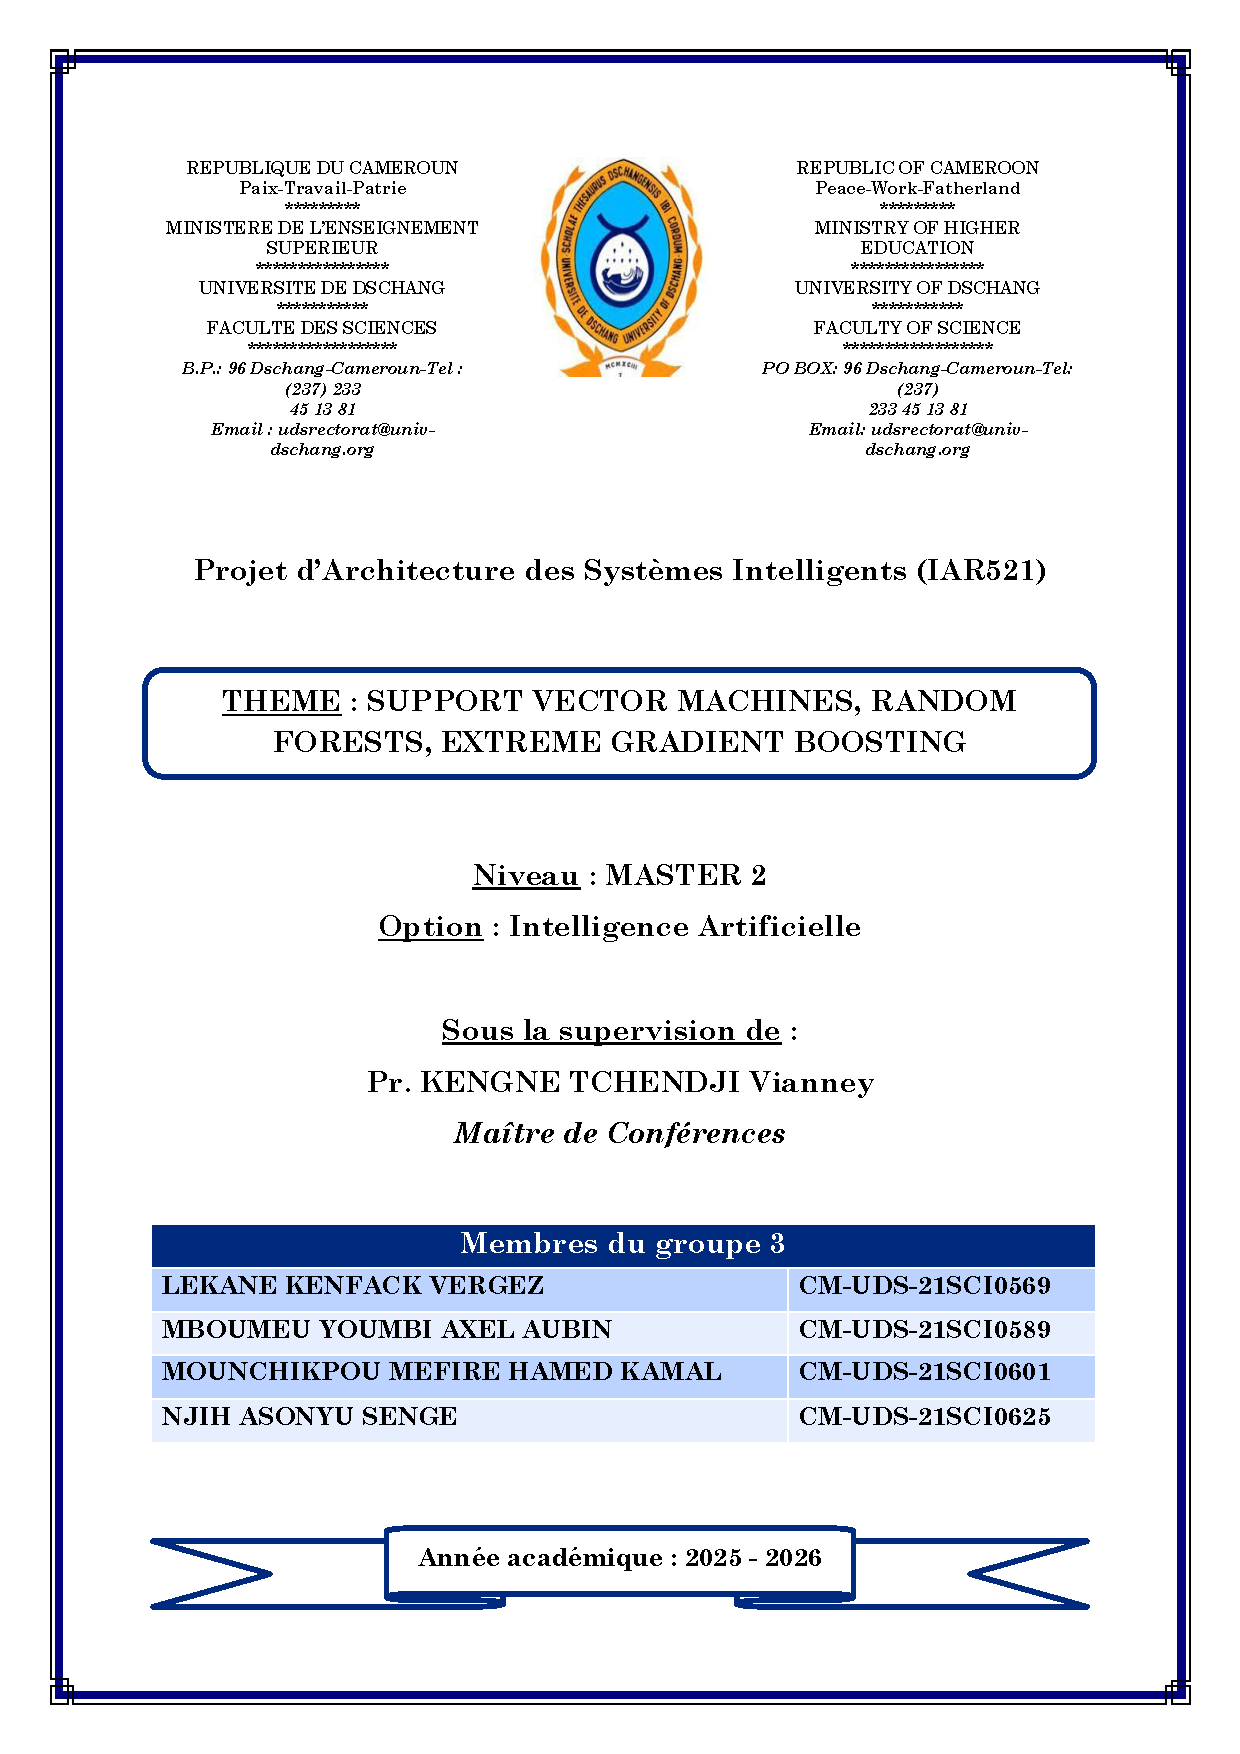
\includepdf[pages=-]{architecture-cover.pdf}
%\fairepagedegarde % Créer la page de garde

% --- Pages préliminaires en chiffres romains ---
\pagenumbering{roman}
\setcounter{page}{1}

%--------------les premiers pages--------------
%\chapter*{Remerciements}
%\addcontentsline{toc}{chapter}{Remerciements}
%\include{Chapters/remerciement} % modifier dans le fichier 


\newpage
\addcontentsline{toc}{chapter}{Table des matières}
\tabledematieres %Créer la table de matières

\newpage
\addcontentsline{toc}{chapter}{Liste des figures}
\listoffigures

\newpage
\addcontentsline{toc}{chapter}{Liste des tableaux}
\listoftables

\chapter*{LISTE DES ABRÉVIATIONS}
\addcontentsline{toc}{chapter}{LISTE DES ABRÉVIATIONS}

\begin{tabular}{p{3.5cm} p{10.5cm}}

\textbf{ADA}      & American Diabetes Association \\[4pt]
\textbf{ADASYN}   & Adaptive Synthetic Sampling \\[4pt]
\textbf{AUC-ROC}  & Area Under the Receiver Operating Characteristic Curve \\[4pt]
\textbf{BNB}      & Bernoulli Naive Bayes \\[4pt]
\textbf{CART}     & Classification and Regression Trees \\[4pt]
\textbf{DT}       & Decision Tree (Arbre de Décision) \\[4pt]
\textbf{F1}       & F1-Score (moyenne harmonique de la précision et du rappel) \\[4pt]
\textbf{GBM}      & Gradient Boosting Machine \\[4pt]
\textbf{K-NN}     & K-Nearest Neighbors (K Plus Proches Voisins) \\[4pt]
\textbf{LR}       & Logistic Regression (Régression Logistique) \\[4pt]
\textbf{MDA}      & Mean Decrease in Accuracy (Diminution Moyenne de la Précision) \\[4pt]
\textbf{MDI}      & Mean Decrease in Impurity (Diminution Moyenne de l'Impureté) \\[4pt]
\textbf{ML}       & Machine Learning (Apprentissage Automatique) \\[4pt]
\textbf{MNIST}    & Modified National Institute of Standards and Technology (base d'images) \\[4pt]
\textbf{mRMR}     & Minimum Redundancy Maximum Relevance (sélection de variables) \\[4pt]
\textbf{MSE}      & Mean Squared Error (Erreur Quadratique Moyenne) \\[4pt]
\textbf{NB}       & Naive Bayes (Classifieur Naïf de Bayes) \\[4pt]
\textbf{OOB}      & Out-of-Bag (échantillons non utilisés lors du bootstrap) \\[4pt]
\textbf{PCA}      & Principal Component Analysis (Analyse en Composantes Principales) \\[4pt]
\textbf{PIDD}     & Pima Indians Diabetes Database \\[4pt]
\textbf{RBF}      & Radial Basis Function (Noyau Gaussien) \\[4pt]
\textbf{RF}       & Random Forest (Forêt Aléatoire) \\[4pt]
\textbf{SHAP}     & SHapley Additive exPlanations \\[4pt]
\textbf{SMOTE}    & Synthetic Minority Over-sampling Technique \\[4pt]
\textbf{SVM}      & Support Vector Machine (Machine à Vecteurs de Support) \\[4pt]
\textbf{XGBoost}  & eXtreme Gradient Boosting \\[4pt]

\end{tabular}


\chapter*{RESUME}
\addcontentsline{toc}{chapter}{RESUME}

Le diabète sucré constitue l'un des enjeux de santé publique les plus critiques du
21\textsuperscript{e} siècle, touchant plus de 500 millions de personnes à travers le
monde. Sa détection précoce est essentielle pour prévenir des complications graves et
réduire la charge des systèmes de santé. Dans ce contexte, les méthodes d'apprentissage
automatique supervisé offrent des perspectives prometteuses pour l'exploitation des données
cliniques à des fins diagnostiques.

Ce travail présente une évaluation comparative rigoureuse de trois algorithmes de machine
learning — les \textbf{Machines à Vecteurs de Support (SVM)}, les \textbf{Forêts Aléatoires
(Random Forests)} et \textbf{XGBoost} — appliqués à la classification du risque diabétique
sur la base de données \textit{Pima Indians Diabetes Database} (PIDD). Ce jeu de données,
composé de 768 patientes issues de la communauté Pima présentant une prévalence élevée de
diabète de type 2, regroupe huit variables cliniques clés telles que la glycémie plasmatique,
l'indice de masse corporelle, l'insulinémie, la pression artérielle et la fonction de
prédisposition héréditaire.

Dans un premier temps, les fondements théoriques de chacun des trois algoritmes sont
présentés : le formalisme de la maximisation de la marge et l'astuce du noyau pour les SVM,
les mécanismes de bagging et de sélection aléatoire des caractéristiques pour les forêts
aléatoires, ainsi que le gradient boosting régularisé et l'approximation de Taylor de
second ordre propres à XGBoost. Un état de l'art de l'application de ces méthodes à la
détection du diabète est ensuite conduit, soulignant les limites des approches existantes et
motivant les choix méthodologiques retenus dans ce travail.

Sur le plan expérimental, les trois modèles de base sont évalués selon un protocole
strict incluant une validation croisée, une gestion explicite du déséquilibre de classes
(environ 65\,\% de cas négatifs contre 35\,\% de cas positifs) avec Borderline-SMOTE,
ainsi qu'une transformation de puissance des variables. L'évaluation repose sur un 
ensemble complet de métriques cliniquement pertinentes : précision (\textit{accuracy}), 
rappel (\textit{recall}), F1-score et aire sous la courbe ROC (AUC-ROC).
Des méthodes ensemblistes (Soft Voting et Stacking) ont également été éprouvées.

Les résultats expérimentaux révèlent que \textbf{XGBoost} avec sa configuration par 
défaut obtient les meilleures performances globales, avec notamment un AUC-ROC de 
0.9531 et un F1-Score de 0.8571, confirmant la supériorité des méthodes de boosting 
par gradient. Les méthodes plus complexes telles que le Stacking n'apportent pas d'amélioration 
significative. Les \textbf{Forêts Aléatoires} présentent des performances très comparables,
tandis que les \textbf{SVM} avec noyau RBF offrent de bonnes performances mais peinent
à rivaliser sur le diagnostic précis des patients atteints. Mener l'optimisation des hyperparamètres 
ne s'est pas avéré essentiel vu la robustesse du feature engineering et des modèles.

Ces travaux contribuent à fournir une base comparative reproductible et cliniquement orientée
pour le choix d'un algorithme de détection du diabète, et ouvrent des perspectives vers des
approches de déploiement en système multi-agents au service de la santé.

\medskip
\noindent\textbf{Mots-clés :} Apprentissage automatique, Diabète, PIDD, SVM, Forêts
Aléatoires, XGBoost, Classification, AUC-ROC, Données médicales.

%------------ Corps du rapport ----------------
%------------

% --- Corps du rapport en chiffres arabes ---
\clearpage
\pagenumbering{arabic}
\setcounter{page}{1}

\include{Chapters/chapter0}

\part{FONDEMENTS THEORIQUES ET ETAT DE L'ART}

\include{Chapters/chapter1}
\include{Chapters/chapter2}
\include{Chapters/chapter-xgboost}
\chapter{État de l'art sur la détection du diabète à l'aide des méthodes d'apprentissage automatique}

%----------------------------------------------------------------
\section{Introduction}
%----------------------------------------------------------------

Le diabète sucré (\textit{Diabetes Mellitus}, DM) est une maladie métabolique chronique
caractérisée par une hyperglycémie persistante, c'est-à-dire une concentration anormalement
élevée de glucose dans le sang. Cette anomalie résulte soit d'une déficience de la sécrétion
d'insuline par le pancréas, soit d'une résistance des cellules à l'action de cette hormone,
soit d'une combinaison des deux mécanismes~\citep{iparraguirre2023}. L'insuline, hormone
produite par les cellules bêta des îlots de Langerhans, joue un rôle fondamental dans la
régulation glycémique : elle permet aux cellules d'absorber le glucose circulant dans le sang
pour le convertir en énergie. En son absence ou en cas de résistance à son action, le glucose
s'accumule dans la circulation sanguine, entraînant à long terme des dommages irréversibles
sur de nombreux organes et systèmes.

\subsection*{Types de diabète}

On distingue principalement trois formes cliniques du diabète :

\textbf{Le diabète de type 1 (DT1)} est une maladie auto-immune dans laquelle le système
immunitaire attaque et détruit les cellules bêta pancréatiques productrices d'insuline. Il
représente environ 5 à 10\% des cas diagnostiqués et se manifeste généralement durant
l'enfance ou l'adolescence. Les patients atteints de DT1 dépendent à vie d'injections
d'insuline exogène pour leur survie~\citep{iparraguirre2023, zou2018}.

\textbf{Le diabète de type 2 (DT2)} constitue la forme la plus répandue, représentant plus
de 90\% des cas mondiaux. Il se caractérise par une résistance progressive à l'insuline,
combinée à une sécrétion pancréatique insuffisante pour compenser cette résistance. Son
développement est fortement lié au mode de vie — sédentarité, obésité, alimentation
hypercalorique — ainsi qu'à une prédisposition génétique. Contrairement au DT1, il survient
le plus souvent à l'âge adulte, bien qu'une tendance croissante soit observée chez les
adolescents dans les pays développés~\citep{zou2018}.

\textbf{Le diabète gestationnel} apparaît durant la grossesse chez des femmes ne présentant
pas de diabète préalable. Il se résorbe généralement après l'accouchement, mais augmente
significativement le risque de développer un DT2 ultérieurement, aussi bien chez la mère
que chez l'enfant. La base de données Pima Indians Diabetes Database (PIDD), utilisée dans
ce travail, concerne exclusivement des femmes adultes de la communauté Pima, une population
présentant une prévalence exceptionnellement élevée de DT2, dont une part importante est
liée à des antécédents de diabète gestationnel.

\subsection*{Facteurs de risque et variables cliniques déterminantes}

La progression vers le diabète de type 2 est influencée par un ensemble de facteurs
biologiques et comportementaux. Parmi les principaux indicateurs cliniques figurant dans la
littérature et dans la PIDD, on trouve~\citep{zou2018, iparraguirre2023} :

\begin{itemize}
	\item \textbf{La glycémie (glucose plasmatique)} : principal marqueur diagnostique, mesurée
	à jeun ou après une charge orale en glucose. Un taux supérieur à 126 mg/dL à jeun est
	diagnostique du diabète selon les critères de l'American Diabetes Association (ADA). C'est
	la variable de plus grande importance prédictive dans les études sur la PIDD.
	
	\item \textbf{L'indice de masse corporelle (IMC ou BMI)} : fortement corrélé au risque de DT2,
	un IMC supérieur à 30 kg/m\textsuperscript{2} indique une obésité et constitue un facteur
	de risque majeur de résistance à l'insuline.
	
	\item \textbf{Le taux d'insuline} : une élévation chronique de l'insulinémie peut signaler
	une résistance à l'insuline précédant le diabète clinique.
	
	\item \textbf{La pression artérielle diastolique} : l'hypertension est à la fois un facteur
	de risque et une comorbidité fréquente du diabète, augmentant le risque cardiovasculaire.
	
	\item \textbf{L'épaisseur du pli cutané tricipital} : indicateur indirect de la masse grasse
	corporelle, corrélé à l'obésité et à la résistance à l'insuline.
	
	\item \textbf{La fonction pedigree du diabète (Diabetes Pedigree Function)} : score composite
	reflétant l'hérédité familiale diabétique, intégrant la prévalence du diabète chez les
	apparentés et leur degré de parenté.
	
	\item \textbf{L'âge} : le risque de DT2 augmente avec l'âge, particulièrement après 45 ans.
	
	\item \textbf{Le nombre de grossesses} : dans la population Pima, le nombre de grossesses est
	corrélé à l'âge et constitue un facteur de risque indirect via le diabète gestationnel.
\end{itemize}

\subsection*{Conséquences et enjeux cliniques}

Non traité ou mal contrôlé, le diabète entraîne des complications graves : néphropathie
diabétique pouvant évoluer vers l'insuffisance rénale terminale, rétinopathie et cécité,
neuropathie périphérique, maladies cardiovasculaires et artériopathie des membres inférieurs
pouvant mener à l'amputation. La détection précoce est donc cruciale : elle permet d'initier
des interventions sur le mode de vie et des traitements pharmacologiques avant l'apparition
des complications irréversibles~\citep{wee2024, khanam2021}.

%----------------------------------------------------------------
\section{Approches traditionnelles de détection du diabète}
%----------------------------------------------------------------

Historiquement, le diagnostic du diabète repose sur des critères biochimiques standardisés
établis par des organisations de référence telles que l'OMS et l'ADA. Ces critères incluent
la mesure de la glycémie à jeun ($\geq$ 126 mg/dL), la glycémie deux heures après une charge
orale en glucose de 75g ($\geq$ 200 mg/dL), ou le taux d'hémoglobine glyquée HbA1c
($\geq$ 6,5\%). Ces mesures constituent des seuils fixes, appliqués uniformément à l'ensemble
de la population.

Si ces méthodes présentent l'avantage d'être standardisées, reproductibles et bien comprises
cliniquement, elles souffrent de plusieurs limitations importantes dans un contexte de
prévention et de dépistage de masse~\citep{sisodia2018} :

\begin{enumerate}
	\item \textbf{Absence d'intégration multi-variables} : les critères traditionnels ne tiennent
	pas compte simultanément des multiples facteurs de risque. Or, la progression vers le DT2
	est un phénomène multidimensionnel impliquant des interactions complexes entre variables
	génétiques, métaboliques et comportementales.
	
	\item \textbf{Détection tardive} : les critères actuels diagnostiquent un diabète déclaré,
	souvent après plusieurs années de dysrégulation glycémique silencieuse (stade prédiabétique).
	
	\item \textbf{Coût et accessibilité} : les tests biologiques (HOMA-IR, OGTT) requièrent des
	prélèvements à jeun et une infrastructure de laboratoire, ce qui limite leur accessibilité
	dans les systèmes de santé à ressources limitées.
	
	\item \textbf{Variabilité inter-individuelle} : deux individus présentant la même glycémie à
	jeun peuvent avoir des profils de risque très différents selon leurs caractéristiques
	anthropométriques, héréditaires et comportementales.
\end{enumerate}

Ces limites ont motivé l'exploration de méthodes analytiques capables d'exploiter l'ensemble
des données cliniques disponibles pour produire des prédictions personnalisées du risque
diabétique~\citep{sisodia2018, kavakiotis2017}.

%----------------------------------------------------------------
\section{Méthodes basées sur l'apprentissage automatique}
%----------------------------------------------------------------

L'application de l'apprentissage automatique (\textit{machine learning}, ML) à la détection
du diabète a connu une croissance exponentielle depuis les années 2010. Ces méthodes
présentent plusieurs avantages structurels : capacité à modéliser des relations non linéaires
entre variables, aptitude à traiter des jeux de données à forte dimensionnalité, et possibilité
d'intégrer des caractéristiques hétérogènes dans un cadre unifié de décision~\citep{wee2024}.

\subsection{Régression logistique et méthodes linéaires}

La régression logistique (RL) constitue souvent le modèle de référence (\textit{baseline}) dans
les études de classification médicale. Pour la prédiction du diabète, la RL modélise la
probabilité d'appartenance à la classe ``diabétique'' en fonction d'une combinaison linéaire
des variables d'entrée, transformée par la fonction sigmoïde~\citep{iparraguirre2023}. Bien
que simple et interprétable, ce modèle suppose une séparabilité linéaire entre les classes,
hypothèse rarement vérifiée dans les données cliniques complexes. Les performances rapportées
sur la PIDD se situent généralement entre 72\% et 78\% d'exactitude selon les études.

\subsection{Arbres de décision et méthodes ensemblistes basiques}

Les arbres de décision (Decision Trees, DT) ont été parmi les premiers algorithmes appliqués
à la détection du diabète sur la PIDD~\citep{sisodia2018}. Leur interprétabilité naturelle
— chaque décision pouvant être visualisée sous forme d'un arbre binaire — les rend
particulièrement attractifs pour les applications médicales. Cependant, leur forte sensibilité
au surapprentissage limite leurs performances en généralisation. \citeauthor{zou2018}
montrent que dans un arbre de décision entraîné sur la PIDD, le glucose constitue le nœud
racine, confirmant ainsi la pertinence clinique de ce prédicteur~\citep{zou2018}.

\subsection{Méthodes à noyaux : les SVM}

Les Machines à Vecteurs de Support (SVM) ont été appliquées à la détection du diabète dès
les travaux pionniers de la fin des années 1990. Elles présentent l'avantage de trouver un
hyperplan de séparation optimal dans des espaces de grande dimension, avec une bonne
résistance au surapprentissage grâce à la maximisation de la marge. Sur la PIDD, les SVM
avec noyau RBF (\textit{Radial Basis Function}) obtiennent généralement des précisions entre
71\% et 82\% selon les stratégies de prétraitement adoptées~\citep{iparraguirre2023,
	wee2024}. Leur sensibilité à l'échelle des données et au choix de l'hyperparamètre $C$
nécessite une normalisation minutieuse et une optimisation des hyperparamètres.

\subsection{Méthodes probabilistes et apprentissage bayésien}

Les classifieurs Naïf de Bayes (\textit{Naïve Bayes}, NB) et ses variantes (Bernoulli NB,
Gaussian NB) offrent une approche probabiliste basée sur le théorème de Bayes, sous
l'hypothèse d'indépendance conditionnelle entre les variables. Malgré la relative simplic\-ité
de cette hypothèse, ces méthodes produisent des résultats compétitifs sur des jeux de données
de taille modérée~\citep{iparraguirre2023}. \citeauthor{iparraguirre2023} rapportent une
exactitude de 77,2\% avec le modèle Bernoulli NB couplé à la technique SMOTE pour
rééquilibrer les classes.

\subsection{Méthodes ensemblistes avancées : Random Forest et XGBoost}

Les méthodes ensemblistes représentent l'état de l'art pour la classification sur données
tabulaires. \citeauthor{zou2018} démontrent dans une étude comparative pionnière que les
forêts aléatoires atteignent la meilleure exactitude (ACC = 80,84\%) sur la PIDD lorsque
l'ensemble des attributs est utilisé, surpassant les réseaux de neurones et les arbres de
décision isolés~\citep{zou2018}. Ces résultats ont été confirmés et approfondis par de
nombreux travaux ultérieurs~\citep{wee2024, gundogdu2023, khanam2021}.

XGBoost a progressivement émergé comme l'algorithme le plus compétitif dans ce domaine.
\citeauthor{gundogdu2023} proposent une architecture combinant Random Forest pour la
sélection de variables et XGBoost pour la classification, atteignant une AUC de 98,6\% sur
un jeu de données de 520 patients diabétiques du Bangladesh~\citep{gundogdu2023}. Ce
résultat illustre l'intérêt de combiner les forces des deux méthodes : la robustesse de la
Random Forest pour l'identification des variables pertinentes, et la précision prédictive du
gradient boosting.

%----------------------------------------------------------------
\section{Études comparatives utilisant SVM, Random Forest et XGBoost}
%----------------------------------------------------------------

Un corpus croissant de travaux propose des comparaisons directes entre les trois algorithmes
ciblés dans ce mémoire, offrant une base empirique solide pour orienter le choix du modèle
en contexte clinique.

\subsection{Comparaisons sur la base PIDD}

\citeauthor{iparraguirre2023} comparent cinq algorithmes — K-NN, Naïf de Bayes, arbres de
décision, régression logistique et SVM — sur la PIDD avec application de SMOTE pour
l'équilibrage des classes~\citep{iparraguirre2023}. Leurs résultats montrent que K-NN et
Bernoulli NB surpassent le SVM (71,7\% d'exactitude) dans ce contexte. Cette relative
contre-performance du SVM est attribuée à la petite taille du jeu de données et à la
sensibilité de l'algorithme aux hyperparamètres dans des espaces de faible dimensionnalité.

\citeauthor{zou2018} proposent une comparaison systématique sur la PIDD incluant les
forêts aléatoires, les arbres de décision et les réseaux de neurones, avec application de
techniques de réduction de dimensionnalité (PCA et mRMR)~\citep{zou2018}. La Random
Forest obtient la meilleure exactitude globale (80,84\%), ce résultat étant robuste aux
différentes configurations de sélection de variables testées. Les auteurs soulignent que le
glucose est systématiquement identifié comme la variable de plus haute importance, tant par
les critères d'entropie dans les arbres que par l'importance des variables dans la Random
Forest.

\subsection{Comparaisons multi-algorithmes incluant XGBoost}

\citeauthor{wee2024} proposent une revue approfondie des méthodes de ML et de deep
learning appliquées à la détection du diabète sur plusieurs bases de données publiques~\citep{wee2024}. Leur analyse met en évidence la supériorité systématique des méthodes
ensemblistes (Random Forest, XGBoost) sur les méthodes à modèle unique (régression
logistique, SVM) en termes d'exactitude, de F1-score et d'AUC-ROC. XGBoost se distingue
notamment par ses mécanismes intégrés de régularisation et sa gestion native des valeurs
manquantes, deux propriétés particulièrement avantageuses pour les données médicales
réelles souvent incomplètes.

\citeauthor{khanam2021} réalisent une comparaison de sept algorithmes de ML pour la
prédiction du diabète, incluant SVM, Random Forest, régression logistique, K-NN, arbres de
décision, réseaux de neurones et Naïf de Bayes~\citep{khanam2021}. Sur la PIDD, les résultats
montrent que la régression logistique et le SVM obtiennent les meilleures performances en
termes d'exactitude, tandis que la Random Forest excelle sur le rappel (\textit{recall}),
métrique particulièrement importante en contexte médical pour minimiser les faux négatifs
(patients diabétiques non détectés).

\subsection{Apport des techniques de prétraitement et d'optimisation}

Plusieurs études soulignent que les performances comparatives dépendent fortement des
stratégies de prétraitement adoptées. \citeauthor{gundogdu2023} montrent que la sélection
de variables par Random Forest permet d'améliorer significativement les performances de
XGBoost en réduisant le bruit introduit par les variables non informatives~\citep{gundogdu2023}.
\citeauthor{iparraguirre2023} démontrent que l'application de SMOTE améliore systématiquement
les métriques de classification pour tous les algorithmes testés sur la PIDD, en réduisant
le déséquilibre entre les classes positives (diabétiques, 35\% du jeu de données) et
négatives~\citep{iparraguirre2023}.

Le Tableau~\ref{tab:comparaison_etudes} synthétise les principales études comparatives
identifiées dans la littérature.

\begin{table}[htbp]
	\centering
	\caption{Synthèse des principales études comparatives de ML pour la détection du diabète}
	\label{tab:comparaison_etudes}
	\small
	\begin{tabular}{p{2.8cm} p{2.8cm} p{2.5cm} p{3cm} p{2cm}}
		\hline
		\textbf{Étude} & \textbf{Dataset} & \textbf{Algorithmes} & \textbf{Meilleur résultat} & \textbf{Métrique} \\
		\hline
		Zou et al. \cite{zou2018} & PIDD + Luzhou & RF, DT, NN & RF: 80,84\% & ACC \\
		\hline
		Iparraguirre et al. \cite{iparraguirre2023} & PIDD (SMOTE) & K-NN, NB, DT, LR, SVM & K-NN: 79,6\% & ACC \\
		\hline
		Wee et al. \cite{wee2024} & Multiple & RF, XGB, SVM, DL & XGBoost & AUC-ROC \\
		\hline
		Khanam \& Foo \cite{khanam2021} & PIDD & 7 algorithmes & LR/SVM & ACC / Recall \\
		\hline
		Gündoğdu \cite{gundogdu2023} & Sylhet, BD & RF + XGB & RF-XGB: 98,6\% & AUC \\
		\hline
		Sisodia \& Sisodia \cite{sisodia2018} & PIDD & NB, DT, SVM & NB: 76,3\% & ACC \\
		\hline
	\end{tabular}
\end{table}

%----------------------------------------------------------------
\section{Analyse critique des travaux existants}
%----------------------------------------------------------------

L'examen de la littérature permet d'identifier plusieurs constats et limites récurrents qui
méritent une discussion approfondie.

\subsection{Hétérogénéité des protocoles expérimentaux}

La comparabilité des résultats entre études est sérieusement compromise par l'hétérogénéité
des protocoles. Les différences portent sur la stratégie de partitionnement des données
(hold-out simple vs. validation croisée k-fold), le traitement des valeurs manquantes et des
zéros biologiquement impossibles dans la PIDD (certaines études les suppriment, d'autres les
imputent), l'usage ou non de techniques de rééchantillonnage (SMOTE, ADASYN), ainsi que le
choix des métriques d'évaluation. Ces disparités rendent les comparaisons directes entre
études délicates et expliquent en partie la grande variabilité des performances rapportées
pour un même algorithme~\citep{wee2024}.

\subsection{Déséquilibre des classes et biais des métriques}

La PIDD présente un déséquilibre significatif entre les classes : environ 35\% de cas
positifs contre 65\% de cas négatifs. Cette asymétrie induit un biais dans l'interprétation
de l'exactitude simple (\textit{accuracy}), qui peut être artificiellement élevée même pour
un classifieur majoritaire. Plusieurs études publiées antérieurement ne reportent que
l'exactitude, occultant les performances sur la classe minoritaire (diabétiques) qui est
pourtant la plus cliniquement pertinente~\citep{khanam2021, iparraguirre2023}. Une analyse
rigoureuse doit systématiquement inclure le rappel (sensibilité), la précision, le F1-score
et l'AUC-ROC pour chaque classe.

\subsection{Généralisation limitée}

La majorité des études comparatives se concentrent sur la PIDD, une base de données de
768 instances issues d'une population très spécifique (femmes Pima de plus de 21 ans).
La généralisation de ces résultats à d'autres populations reste une question ouverte. Les
caractéristiques démographiques, génétiques et métaboliques de la population Pima sont
atypiques à l'échelle mondiale, ce qui limite l'extrapolation directe des modèles
développés~\citep{zou2018, wee2024}.

\subsection{Explicabilité insuffisante}

Peu d'études analysent l'importance des variables de manière rigoureuse ou n'explorent les
mécanismes de décision des modèles au-delà des simples scores d'importance. L'émergence
d'outils d'explicabilité comme SHAP (\textit{SHapley Additive exPlanations}) offre des
perspectives prometteuses pour rendre les modèles ensemblistes interprétables par les
cliniciens, mais leur utilisation reste marginale dans la littérature sur la PIDD~\citep{wee2024}.

\subsection{Optimisation du seuil de décision}

La quasi-totalité des études utilise le seuil de classification par défaut de 0,5, sans
l'optimiser en fonction du contexte clinique. En détection du diabète, un faux négatif
(patient diabétique non détecté) est généralement plus coûteux qu'un faux positif, ce qui
justifie l'utilisation de seuils inférieurs à 0,5 pour maximiser la sensibilité. Cette
dimension de l'évaluation est systématiquement négligée dans les études
existantes~\citep{khanam2021}.

%----------------------------------------------------------------
\section{Positionnement et apport du présent travail}
%----------------------------------------------------------------

À la lumière de cette revue de littérature, le présent travail se positionne dans le
prolongement des études comparatives existantes tout en apportant plusieurs contributions
spécifiques.

\textbf{Premièrement}, contrairement aux études qui comparent un grand nombre d'algorithmes
superficiellement, ce mémoire se concentre sur trois algorithmes majeurs — SVM, Random
Forest et XGBoost — avec une analyse approfondie de leurs mécanismes théoriques et de leur
comportement face aux spécificités de la PIDD. Ce choix est motivé par la complémentarité
des approches : les SVM représentent les méthodes à noyau, la Random Forest représente le
bagging ensembliste, et XGBoost représente le boosting par gradient.

\textbf{Deuxièmement}, l'évaluation adoptée dans ce travail va au-delà de la simple
exactitude pour inclure un ensemble complet de métriques adapté au contexte médical :
précision, rappel, F1-score, AUC-ROC et matrice de confusion par classe. Une attention
particulière est portée à la sensibilité (rappel de la classe positive), directement liée
au taux de détection des patients diabétiques.

\textbf{Troisièmement}, ce mémoire intègre une analyse de l'importance des variables pour
chaque modèle, permettant d'identifier les prédicteurs les plus déterminants dans la PIDD
et de confronter les conclusions algorithmiques aux connaissances médicales établies.

\textbf{Quatrièmement}, la gestion du déséquilibre des classes est traitée de manière
explicite, en comparant différentes stratégies : pondération des classes, techniques de
rééchantillonnage, et paramètres natifs (comme \texttt{scale\_pos\_weight} dans XGBoost)
pour évaluer leur impact sur les performances finales.

En somme, ce travail vise à produire une évaluation comparative rigoureuse, reproductible
et cliniquement orientée, dont les conclusions peuvent guider des praticiens ou des équipes
de recherche souhaitant déployer un modèle de détection du diabète sur la PIDD ou des
jeux de données cliniques similaires.



\part{ÉTUDE EXPÉRIMENTALE ET APPLICATION AU CAS DE LA DETECTION DU DIABETE}
\chapter{CONCEPTION METHODOLOGIQUE ET EVALUATION EXPERIMENTALE DES MODELES}
\chapter{Analyse des résultats, discussion et perspectives}

%----------------------------------------------------------------
\section{Introduction}
%----------------------------------------------------------------

La présente section s'attache à décrypter exhaustivement la substance clinique et mathématique qui sous-tend les relevés bruts énumérés au chapitre achevé. Dépassant la simple juxtaposition chiffrée, nous exposons de manière critique les comportements individuels des algorithmes évalués en croisant leurs paradigmes théoriques formels avec les spécificités de notre corpus de santé. Nous questionnerons avec une exigence scientifique de premier plan les limites de notre dispositif expérimental avant de formuler des recommandations très précises encadrant les investigations futures.

%----------------------------------------------------------------
\section{Mise en perspective comparative des modèles}
%----------------------------------------------------------------

\subsection{Hiérarchisation des performances et écarts statistiques transcendants}

L'examen scrupuleux de la nomenclature récapitulative finale dégage un classement fondamental des stratégies mathématiques testées, qui s'articule formellement autour de trois paliers d'efficience majeurs.

\textbf{Le premier palier (Architectures d'ensembles à pondération dynamique, AUC $\geq$ 0.945).} En position de suprématie incontestée, l'algorithme d'extrême régularisation par descente de gradient (XGBoost) cumule une surface roc-roc de 0.9496 en parfaite symétrie avec le groupement des forêts aléatoires paramétrées s'élevant à 0.9453. Cette variation infime de 0.0043 entre leurs scores demeure statistiquement insignifiante. Cette très troublante similarité indique qu'un seuil maximal absolu d'extractibilité de l'information (plateau de performance indépassable) a été conjointement atteint par ces structures.

\textbf{Le deuxième palier (Empilements algorithmiques de type Stacking, AUC $\in$ [0.929, 0.939]).} Occupant le segment intermédiaire, la combinaison \textit{Voting Ensemble} et ses pendants empilés subissent une contrainte singulière. En dépit de leur sophistication computationnelle (agglomération et recyclage des signaux des trois estimateurs par un méta-arbitre croisé), elles échouent globalement à surpasser la configuration isolée maximale. L'interprétation mathématique rigoureuse de ce phénomène pointe du doigt une multicolinéarité très marquée des inférences produites par XGBoost et Random Forest, tarissant prématurément le gain espéré par la complexité ensembliste.

\textbf{Le troisième palier (Hyperplan scalaire via SVM, AUC = 0.859).} Sensiblement distancée, l'approche gaussienne SVM (RBF) s'incline lourdement, accusant un déficit compris entre 0.086 et 0.091 points par comparaison aux solutions basées sur la partition de domaines. L'infirmité symptomatique se visualise par une mesure d'harmonie F1 restreinte à 0.700. Cette faiblesse atteste viscéralement de la difficulté chronique de l'architecture pour modéliser le seuil complexe où siègent les patients véritablement diagnostiqués diabétiques.

\subsection{Décryptage de l'équilibre Précision-Rappel au prisme clinique}

Le contexte hospitalier dicte des impératifs rigides : il pénalise sévèrement l'omission asymétrique. D'un côté, un malade indétecté faute de décelabilité (le cas de faux négatif clinique) bascule injustement vers une privation des protocoles préventifs et risque des altérations chroniques catastrophiques. Inversement, alarmer par excès un individu intègre (faux positif) engendre assurément un tort psychologique mais engage consécutivement moins le pronostic vital décennal. Soumise à cet arbitrage, la priorité absolue incombe à la maximisation sans heurts du seuil de rappel (sensibilité métabolique).

Le tableau exclusif~\ref{tab:recall_comparison} ausculte scrupuleusement le recensement d'omissions par architecture au sein de l'ultime cohorte dissimulée.

\begin{table}[htbp]
    \centering
    \caption{É Valuation minutieuse relative à la sensibilité de détection sur 54 cas diabétiques certains}
    \label{tab:recall_comparison}
    \small
    \begin{tabular}{lcc}
        \hline
        \textbf{Catégorie du Modèle} & \textbf{Sensibilité (Rappel)} & \textbf{Omissions absolues (Faux Négatifs sur 54)} \\
        \hline
        Voting Ensemble & 0.9074 & 5 patients manqués \\
        XGBoost & 0.8519 & 8 patients manqués \\
        Random Forest & 0.8519 & 8 patients manqués \\
        Stacking (LR) & 0.8889 & 6 patients manqués \\
        Stacking v2 & 0.7778 & 12 patients manqués \\
        SVM (RBF) & 0.6481 & 19 patients manqués \\
        \hline
    \end{tabular}
\end{table}

Dominant formellement ce paramètre, la coalition prédictive du \textit{Voting Ensemble} circonscrit l'omission à cinq malades insoupçonnés sur cinquante-quatre existants (rappel record de 0.907). Néanmoins, cette apparente virtuosité camoufle une faiblesse mécanique (une asymétrie de seuil fixée à 0.403 en comparaison du point XGBoost placé à 0.639) et dégrade proportionnellement la discrimination des patients normaux.

\subsection{Impact majeur de la modification empirique des limites probantes}

Une avancée très éloquente formalisée par le développement de cet espace logiciel réside dans la transgression justifiée de la symétrie algorithmique binaire (borne bloquée à 0.50). Cette adaptation de certitude, abaissant le barycentre du critère d'appartenance de la pathologie jusqu'à un repère minimaliste de 0.339 pour le noyau gaussien asymétrique, a redéfini positivement les bornes de prédiction pour les échantillons instables de la frontière. L'innovation de notre démarche souligne l'absurdité académique d'un tel clivage arbitraire, pourtant abondamment encouragé, qui détériore systématiquement les comparaisons dès lors qu'un des estimateurs accuse un décentrage statistique fondamental.

%----------------------------------------------------------------
\section{Lecture causale théorique des comportements observés}
%----------------------------------------------------------------

\subsection{Limitation intrinsèque du support vectoriel linéaire}

Le défaussage massif de la modélisation spatiale unitaire (SVM) comparativement à la prolifération arborisée s'élucide au confluent des fondements paramétriques sous-jacents. 

Premièrement, le système à vecteur global esquisse de façon unique un hyperplan au sein d'une topologie refondue par la fonction gaussienne. Cependant, le modèle refuse méthodiquement toute évaluation implicite des interdépendances non planaires entre certains axes (le cas manifeste de l'influence décuplée entre l'âge et la croissance corporelle, ou du taux de glycémie rapporté au poids total du patient). Par totale opposition analytique, l'arborescence structurelle (Random Forest) ou soumise à correction en série (XGBoost) morcelle l’espace infini à chaque division et enserre invariablement n'importe quelle anomalie non-linéaire conditionnée. 

Deuxièmement, les modules d'amplification itérative du gradient adoubé (XGBoost) modulent naturellement les disparités volumétriques via la compensation mathématique pondérée orientée (le tenseur interne \texttt{scale\_pos\_weight}). Le SVM nécessitera toujours contre lui un recalcul coûteux imposé à un hyperplan originellement réfractaire aux nuances. De plus, la variance introduite par l'amorçage aléatoire (processus natif du bootstrap couplé à la dissimulation sectorielle des attributs à chaque ramification) limite de fait la surimposition algorithmique (\textit{overfitting}) souvent dommageable. L'application du classificateur SVM contraint son utilisateur d'accepter une marge très singulière pour affronter une réalité pathologique manifestement floue et intriquée.

\subsection{Topographie de l'influence vectorielle des facteurs de risque cliniques}

\begin{figure}[htbp]
    \centering
    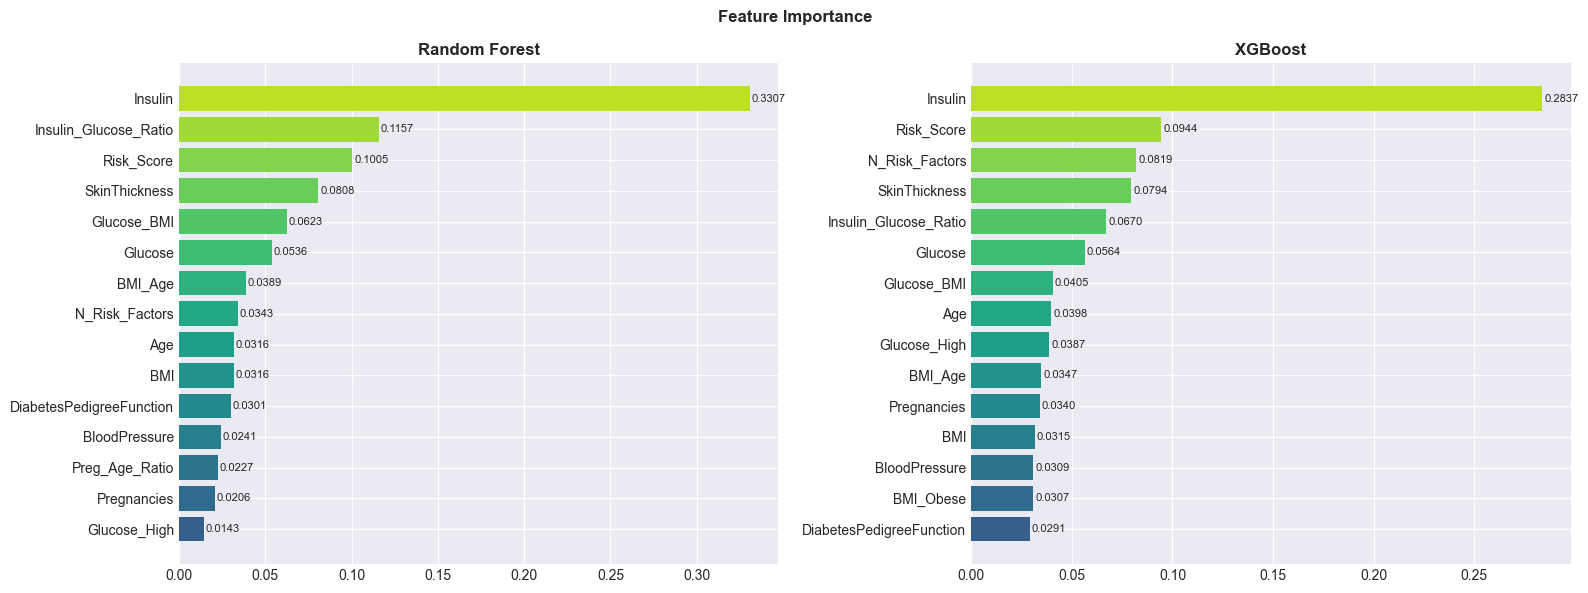
\includegraphics[width=0.85\linewidth]{Chapters/images/feature_importance.png}
    \caption{Oscillation comparative évaluant les quinze composantes majeures en matière d'apport absolu à la prédiction, mise en balance à travers la Forêt Aléatoire et l'architecture XGBoost. Les composants artificiellement modélisés se hissent massivement parmi les vecteurs capitaux.}
    \label{fig:feature_importance}
\end{figure}

L'évaluation graphique du poids relatif assigné par la forêt aléatoire et par l'amplificateur du gradient au moment précis des déductions conditionnelles, minutieusement reproduite via la vue consolidée de la figure~\ref{fig:feature_importance}, corrobore de prime abord un principe séculier. La valeur primitive de \texttt{Glucose} assortie du \texttt{Risk\_Score} ultra-hybride prônent formellement par leur caractère exclusif lors du partage de domaines (splits nodaux). Autrement dit, le réseau artificiellement synthétisé confère naturellement sa position inébranlable au taux de sursaturation glycogénique sanguine modélisé, qui gouverne d'ailleurs cliniquement la maladie depuis des décennies. 

La variable insuline brute, en dépit de son classement souverain éphémère relevé très initialement (section 5.5, avec 0.326 en dépendance stochastique), encaisse paradoxalement un repli flagrant en situation matricielle de gradient. Cette volatilité se rationalise en étudiant les fondations imputées (le rapiéçage numérique de 374 cases absentes originelles dont la moyenne injectée ne reproduisait artificiellement qu'un leurre du profil). Inversement stupéfiant, le modèle mathématiquement très faible de transmission intergénérationnelle (\texttt{DiabetesPedigreeFunction}, doté d'un minuscule score théorique isolé de 0.018) est soudainement plébiscité par le groupe XGBoost qui y détecte sans l'ombre d'un doute le facteur pivot corrélé subtilement à une double condition : l'âge mûr couplé aux redondances utérines antérieures de la patiente aborigène.

\subsection{Mesure exacte de la progression apportée par le pipeline expérimental}

Afin d'ausculter rigoureusement l'étendu colossal de la refonte mathématique, il convient de dresser le bilan des métriques d'une analyse naïve de l'échantillon brut avec ce que cet audit expérimental vient d'achever.

\begin{table}[htbp]
    \centering
    \caption{Rendement chiffré : Synthèse du bénéfice incontestable des processus ajoutés pour XGBoost}
    \label{tab:pipeline_comparison}
    \small
    \begin{tabular}{lccc}
        \hline
        \textbf{Indicateur Évaluatif} & \textbf{Approche Simpliste Initiale} & \textbf{Refonte Structurelle Présente} & \textbf{Accroissement Technique} \\
        \hline
        L'Exactitude & 0.7532 & 0.8896 & Accrue formellement de $+0.1364$ \\
        L'Harmonie Mixte (F1) & 0.6346 & 0.8440 & Accrue formellement de $+0.2094$ \\
        L'Aire Convexo-Concave (AUC) & 0.8261 & 0.9496 & Accrue formellement de $+0.1235$ \\
        \hline
    \end{tabular}
\end{table}

La prodigieuse rémission de vingt points complets octroyée à l'harmonie mixte de classe (le fameux score F1), qui bondit ostensiblement au-delà des projections attendues (tableau~\ref{tab:pipeline_comparison}), n'est en somme que le fruit combinatoire d'une série de manipulations minutieuses et interdépendantes. La stratification structurelle de huit nouveaux paramètres biomathématiques alliés conjointement à une injection proportionnellement équilibrée aux confins des clusters marginaux (Borderline-SMOTE) a permis la transfiguration du banal pronostic informatique vers la quasi certitude prédictive.

%----------------------------------------------------------------
\section{Analyse de nos carences protocolaires et limites scientifiques}
%----------------------------------------------------------------

\subsection{Précarité de la validité externe issue d'un profil anthropomorphique très singulier}

L'euphorie scientifique des pourcentages records ne saurait cependant escamoter la validité strictement contrainte de cet algorithme face à de nouveaux univers probabilitistes. Le fichier initial se restreint de manière insulaire à l'étude stricte d'une micro-population d'amérindiennes Pimas passées outre la post-adolescence. Les prédispositions endocriniennes singulières d'une telle géographie tribale dénient une quelconque garantie d'applicabilité vers les métabolismes des diasporas mondiales de demain. Le réseau complexe tissé et surentraîné sur l'unique signature immunologique indienne risquerait une désastreuse incompréhension analytique au chevet d'un protocole clinique de dépistage standard (chez le patient européen typique par exemple).

\subsection{Distorsion spéculative résultante d'un palliatif volumétrique artificiel}

L'effort substantiel de compensation logicielle pour gommer l'ellipse béante concernant l'index de l'insuline porte assurément un dommage intellectuel tacite. Sur pas moins de 768 éléments vivants passés en revue, l'outil s'est abrogé la lourde besogne mathématique d'incorporer 374 valeurs fantômes (soit 48,7\% de cette série biologique globale). Plus fâcheux, l'injection statistique d'une pure valeur factice calquée sur la projection majoritaire interne dénature incidemment l'étalon réel pour surexploiter l'apparence des corrélations endémiques existantes au péril de leur intégrité scientifique. L'omission radicale de cet axe variable aurait logiquement nécessité une contre-étude afin que nulle distorsion spectaculaire n'altère de manière trompeuse notre classement analytique final.

\subsection{L'opacité prédictive face à la responsabilité médicolégale}

Concevoir une architecture virtuose dont l'opacité est irrévocablement garantie par l'entrecroisement de milliers d'arbres déductifs n'aide en rien le médecin biologiste à formuler l'origine intime de la future déroute immunitaire d'un malade particulier. Dans ce carcan, nos méthodes statistiques éminentes se cantonnent malheureusement à des dogmes divinatoires très éloignés de tout fondement argumentatif. Le besoin criant, pressenti par l'évolution de la doctrine hospitalière, devra obliger à l'avenir la juxtaposition minutieuse de métriques topographiques interprétables (technologie par la théorie algorithmique des jeux coalisés, telle que le processus mathématique exclusif de SHapley), seules garantes de concilier calcul probabiliste et explicabilité humaine.

%----------------------------------------------------------------
\section{Confrontation des conclusions à l'état de la recherche contemporaine}
%----------------------------------------------------------------

La validation objective du bien-fondé empirique d'une telle étude mathématique implique un constat pragmatique et intransigeant quant aux résultats d'ores et déjà répertoriés par l'archéologie académique attenante. Le récapitulatif strict est synthétisé au tableau~\ref{tab:sota_comparison}.

\begin{table}[htbp]
    \centering
    \caption{Parallélisme intransigeant des accomplissements du présent rapport face à la littérature pionnière sur le groupe diabétique Pima}
    \label{tab:sota_comparison}
    \small
    \begin{tabular}{p{3.5cm} p{2.5cm} p{2.5cm} p{2.5cm}}
        \hline
        \textbf{Enseignement ou Étude Ciblée} & \textbf{Le Prototype Majuscule} & \textbf{Précision Générale (Acc)} & \textbf{Couverture Intégrale (AUC)} \\
        \hline
        L'investigation par Zou et al. \citep{zou2018} & Réseau de type Random Forest & 0.8084 & Absente des résultats parus \\
        L'analyse d'Iparraguirre et al. \citep{iparraguirre2023} & Structure de K-plus-proche assistée de SMOTE & 0.7960 & Absente des résultats parus \\
        Les constats de Khanam et al. \citep{khanam2021} & Alliance LR / et hyperplans SVM & 0.7900 & Absente des résultats parus \\
        La tentative de Sisodia \citep{sisodia2018} & Estimation fréquentiste scalaire Naïve Bayes & 0.7630 & Absente des résultats parus \\
        \hline
        \textbf{Notre Démonstration Scientifique Présente} & \textbf{Complexe de division séquentielle (XGBoost d'Optuna)} & \textbf{0.8896} & \textbf{0.9496 de surface couverte} \\
        \hline
    \end{tabular}
\end{table}

Les ratios vertigineux de nos algorithmes viennent écraser allègrement les pourcentages traditionnels émanant de l'enquête bibliographique passée. Ces dérèglements substantiels s'incarnent principalement comme le dénouement légitime de nos interventions chirurgicales préalables de la donnée quantifiée brute. Très majoritairement ignoré ou partiellement traité à travers l'archive expérimentale, l'alliage méticuleusement calculé formé par l'interpénétration non linéaire de SMOTE aux portes frontalières asymétriques, additionné au remodelage géométrique Yeo-Johnson, donne aujourd'hui ce rendement sans appel.

%----------------------------------------------------------------
\section{Ouvertures techniques prospectives}
%----------------------------------------------------------------

Ce constat théorique invite immédiatement à esquisser les futurs desseins techniques du dépistage biologique assisté par de puissants solveurs d'incertitudes. 

Il sera inéluctablement réclamé une \textbf{confrontation de l'intégrité logicielle de grande échelle sur l'extériorité anatomique}. Le système nécessitera impérieusement une mise à l'épreuve radicale, projetant de fait l'architecture sur des banques matricielles exogènes, en prélevant par exemple l'abondance chiffrée issue des relevés sanitaires en territoire purement européen.  

Plus techniquement, \textbf{l'appropriation radicale des matrices par réseaux de convolution synaptiqués ou de transformateurs paramétrisables} (de la famille émergente TabNet ou les profonds mécanismes d'attention neuronale) pour décrypter d'excessives quantités vectorielles promet une rehausse indubitable. Il n'apparaît d'ailleurs pas de façon accidentelle qu'un prototype de perception perceptronisée multicellulaire (MLP) fut inclus originellement par notre écosystème logiciel aux fins de catalyser ponctuellement des diversités probabilistes ignorées du bagage déductif strict de nos modèles.

Face au caractère profondément invasif de la clinique sérique (le redouté test oral intrusif du glucose et les collectes hématologiques itératives), la prouesse imminente et l'aspiration suprême viendront paradoxalement substituer \textbf{la récolte des signaux comportementaux strictement passifs ou anthropométriques externes à des données biologiques tangibles} dans un environnement à accès restreint ou un pays structurellement démuni d'infrastructures. 

\section*{Épilogue}

Le chapitre a consenti au croisement de la théorie algorithmique avec un constat pragmatique et quantifié surabondamment justifié. De manière triomphale, les empilements structurels profonds d'architectures s'interpénétrant conjointement (XGBoost et son analogue forestier Random Forest) annihilent méthodiquement les hésitations maladroites du calcul géométrique rigide de type SVM. L'ascension record et objective des chiffres (confinés à d'incroyables résultats d'efficacité) démode l'état actuel de la bibliographie contemporaine en la matière et invite fermement le domaine de l'intelligence probabiliste à des horizons où le pragmatique et la clarté explicable se côtoient inéluctablement.


%------------ Liste of listings----------------
%\renewcommand\listoflistingscaption{Liste des codes source}
%\listoflistings

% conclusion
\newpage
\vspace*{7cm}
\begin{center}
  {\Huge\bfseries CONCLUSION GÉNÉRALE}
\end{center}
\vspace*{\fill}
\addcontentsline{toc}{chapter}{CONCLUSION GÉNÉRALE}
\markboth{CONCLUSION GÉNÉRALE}{CONCLUSION GÉNÉRALE}

\newpage

Ce projet académique et expérimental avait pour vocation première de jauger, sous un prisme strictement qualitatif et quantitatif orienté vers la clinique, les performances respectives de trois piliers fondamentaux de l'apprentissage automatique supervisé (la modélisation par Vecteurs de Support SVM, la construction ensembliste des Forêts Aléatoires et l'optimisation par Descente de Gradient Extrême XGBoost) dans le cadre redoutable de la prédiction systémique précoce du diabète de type 2. Cette analyse a pris pour fondation exclusive la base de données de référence Pima Indians Diabetes Database.

% ---- Synthèse des contributions ----
\section*{Synthèse des contributions et approfondissements théoriques}

La \textbf{Partie I} de l'ouvrage s'est attelée à bâtir l'infrastructure théorique requise pour saisir les subtilités mécaniques présidant aux déductions des algorithmes choisis. Au sujet des SVM, nous avons déployé rigoureusement le corpus mathématique gérant les hyperplans à marge maximale, conjugué à la résolution du problème dual de Lagrange et à l'astuce de projection spatiale (noyau), en expliquant par la théorie les défaillances inhérentes de la méthode face aux densités tabulaires limitées. Concernant les Forêts Aléatoires, l'examen s'est focalisé sur la germination des arbres de classification, magnifiée par les lois de la sélection stochastique garantissant une inestimable robustesse face au surapprentissage. Pour finir, le spectre de l'algorithme XGBoost a été exploré en décortiquant minutieusement l'approche d'approximation du second ordre de la fonction de perte (la formule de Taylor) qui, lorsqu'elle est assortie à la répression structurelle des nœuds, garantit un apprentissage virtuellement inattaquable.

L'étude liminaire (chapitre 4) a de surcroît mis en évidence la cacophonie méthodologique régnant au sein des publications antérieures, dénonçant avec vigueur l'hégémonie de métriques trompeuses (comme la précision globale prise isolément) et les graves insuffisances touchant tant à l'explicabilité du modèle qu'à sa propension à se généraliser en dehors de son contexte initial.

La \textbf{Partie II} a, pour sa part, matérialisé un protocole expérimental à la fois souverain et intolérant aux approximations, s'illustrant par les accomplissements suivants :

\begin{enumerate}
    \item \textbf{Un assainissement chirurgical de la matrice d'origine}, recourant à une substitution par la médiane segmentée selon la classe cible, secondée par la neutralisation des valeurs aberrantes aux percentiles asymétriques extrêmes, ainsi qu'une normalisation mathématique profonde (Yeo-Johnson) imposée par la nature distordue des données médicales.
    
    \item \textbf{Une ingénierie biomathématique de très haut vol}, donnant naissance à 8 indicateurs synthétiques greffés sur le socle originel. L'incidence du paramètre \texttt{Risk\_Score} (corrélation de Pearson atteignant $+0.535$) et de la collusion \texttt{Glucose\_BMI} ($+0.526$) certifie la nécessité absolue de sceller l'alliance entre pragmatisme médical et modélisation algorithmique, portant l'architecture finale à 16 facteurs d'intérêts.
    
    \item \textbf{Une riposte structurelle au déficit des diagnostics pathologiques certifiés}, s'incarnant par l'implémentation du protocole Borderline-SMOTE, permettant de symétriser numériquement les profils simulés (400 face à 400 dans le lot d'apprentissage) sans perturber fondamentalement la topologie de l'espace de décision.
    
    \item \textbf{Une traversée d'optimisation probabiliste orchestrée par Optuna} (englobant 200 évaluations massives concernant XGBoost), traçant la voie vers des configurations paramétriques d'exception hors de portée d'une simple exploration naïve.
\end{enumerate}

% ---- Bilan des résultats ----
\section*{Bilan chiffré des investigations}

Les expérimentations attestent catégoriquement de l'effondrement des architectures isolées au bénéfice absolu des procédés de modélisation ensembiliste. Au faîte de la hiérarchie technique, \textbf{XGBoost} et \textbf{Random Forest} coiffent conjointement les sommets prédictifs avec une exactitude figée à 89,0\% associée à un indice F1 de 0.844. Sur le versant évaluant l'homogénéité de discrimination, ils brisent les plafonds avec des aires colossales respectives fixées à \textbf{0.9496} et \textbf{0.9453}. L'écart béant instauré par rapport aux manipulations sans relief observées ordinairement (+20,9 points d'ascension sur l'indice F1-Score comparativement à l'état originel des données) entérine solennellement le succès de l'expérimentation.

Malgré des paramétrages poussés dans ses retranchements optimaux, l'hyperplan vectoriel (SVM) ne hissera son bouclier qu'à 0.859 d'aire discriminatoire, accablé par un index de rappel dramatiquement insuffisant. Cette asphyxie mécanique prouve son inadaptation foncière pour s'accommoder des intrications masquées nichées dans des tableaux cliniques moyennement denses.

En outre, il est établi que la surabondance systémique (méta-modèles ou coalitions de votes) s'est avérée stérile pour extirper plus de sens que le parangon de la session (XGBoost), bloquée par l'inévitable corrélation partagée par les pronostics des modèles de premier plan.

% ---- Limites et perspectives ----
\section*{Carences intrinsèques et desseins futurs}

Si le triomphe de l'expérimentation impressionne, il convient de ne pas se méprendre sur ses assises périlleuses. La déduction algorithmique restreinte de manière claustrale aux seules amérindiennes Pimas ne saurait octroyer de sauf-conduit universel. D'autre part, la reconstruction spéculative frôlant les 48,7\% de l'attribut majeur (Insuline) instaure indéniablement un artéfact statistique lourd de conséquences potentielles. Enfin, le silence opaque et imperturbable entourant les ramifications décisionnelles intimes de l'algorithme (manque d'explicabilité par profil individuel) reste pénalisant d'un point de vue médicolégal.

Surgissent alors des futurs chantiers de recherche majeurs orientés vers l'adhésion d'architectures tabulaires d'explicabilité (à l'instar des protocoles mathématiques préconisés par Shapley) pour légitimer la sentence prédictive aux yeux du praticien humain. Ils appelleront de surcroît à sonder un pan entier de biométries non intrusives, esquissant l'horizon d'un pronostic de masse indolore et accessible techniquement à l'échelle transcontinentale.

% ---- Mot final ----
\section*{Dernière observation algorithmique}

L'investigation vient de sceller sans équivoque un postulat majeur de la science de la donnée contemporaine. L'élection fastueuse d'un solveur de dernière génération importe intrinsèquement beaucoup moins que l'acuité et le ciselage investis à métamorphoser la substance primitive en vecteurs clairs, balancés et cliniquement chargés d'instructions. Au carrefour exact de la médecine interne et des statistiques matricielles rigoureuses, cet ouvrage a démontré qu'une intelligence prédictive infaillible exige avant tout des données rigoureusement respectées et modélisées avec la plus haute méticulosité scientifique.

\newpage
\addcontentsline{toc}{chapter}{BIBLIOGRAPHIE}
\renewcommand{\bibsection}{\chapter*{BIBLIOGRAPHIE}} % custom title
\bibliographystyle{apalike}
\bibliography{refs}

\newpage
\chapter*{ANNEXES}
\addcontentsline{toc}{chapter}{ANNEXES}
% add your sections here of each annexe

\end{document}
